% Template for ICASSP-2015 paper; to be used with:
%          spconf.sty  - ICASSP/ICIP LaTeX style file, and
%          IEEEbib.bst - IEEE bibliography style file.
% --------------------------------------------------------------------------
\documentclass{article}
\usepackage{spconf,amsmath,graphicx}
\usepackage{amsfonts}

% Example definitions.
% --------------------
\def\x{{\mathbf x}}
\def\L{{\cal L}}

% Title.
% ------
\title{Modulation Design in Amplify-and-Forward Two-Way Relay HARQ Channel}
%
% Single address.
% ---------------
\name{Author(s) Name(s)\thanks{Thanks to XYZ agency for funding.}}
\address{Author Affiliation(s)}
%
% For example:
% ------------
%\address{School\\
%	Department\\
%	Address}
%
% Two addresses (uncomment and modify for two-address case).
% ----------------------------------------------------------
%\twoauthors
%  {A. Author-one, B. Author-two\sthanks{Thanks to XYZ agency for funding.}}
%	{School A-B\\
%	Department A-B\\
%	Address A-B}
%  {C. Author-three, D. Author-four\sthanks{The fourth author performed the work
%	while at ...}}
%	{School C-D\\
%	Department C-D\\
%	Address C-D}
%
\begin{document}
%\ninept
%
\maketitle
%
\begin{abstract}
  % (what we do)
  As a practical transmission enhancement technique for relay and HARQ system,
  Modulation Diversity (MoDiv) uses distinct mappings to the same constellation
  for different (re)transmissions. 
  % (how they do)
  % (how we do)
  In this work, we study the MoDiv optimization
  in a Amplify-and-Forward (AF) Two-Way Relay Channel (TWRC). The design of
  MoDivto minimize the bit-error rate (BER) is formulated into a successive
  Koopmans-Beckmann Quadratic Assignment Problem (QAP), which is solved
  sequatially with a robust taboo search method.
  % (main results)
  The performance gain of our MoDiv scheme over retransmission without remapping
  and a heuristic MoDiv scheme is demonstrated with numerical ressults.
\end{abstract}
%
\begin{keywords}
  Modulation diversity, two-way relay, amplify-and-forward, HARQ, QAP
\end{keywords}
%
\section{Introduction}
\label{sec:intro}

% Motivation and literature review for Two-way relay-HARQ. HARQ first,
% then two-way relay
As an advanced technique to improve the robustness of high-rate wireless
transmissions against poor channel conditions, Hybrid Automatic Repeat reQuest
(HARQ) has found its application in various communication
systems~\cite{cripriano2010overview}. HARQ works on both PHY layer and MAC
sublayer to mitigate packet loss due to channel fading and
link-adaptation accuracy. Recently, substantial research interest
has been drawn to HARQ in Two-Way Relay Channel
(TWRC) [2-4].
In~\cite{iannello2009throughput}, the average throughput of naive Type-I HARQ
policy for both Amplify and Forward (AF) and Decode and Forward (RF) TWRC schemes have
been analyzed. The energy-delay tradeoff, and the diversity-multiplexing
tradeoff of type-II HARQ policy, also known as full Incremental Redundancy (IR),
for AF TWRC scheme have been studied in~\cite{choi2013energy}
and~\cite{xu2014diversity}, respectively. Related works about TWRC with ARQ
for different relay schemes and retransmission policies can also be
found in~\cite{popovski2007wireless, chen2012arq, guan2015twoway} and the references therein.

% Literature review on MoDiv for HARQ-CC
Apart from the naive Type-I HARQ and HARQ-IR, Type-I HARQ with maximal ratio
combining (MRC), also known as HARQ-Chase Combining
(HARQ-CC)~\cite{chase1985code}, is another simple and practical HARQ
scheme supported by such standands as HSPA~\cite{TS25.308},
LTE~\cite{sesia2009lte} and so forth. As practical transmissions often admit
linear modulations of finite-alphabet constellation (e.g. Q-ary QAM), the
performance of HARQ-CC can be improved with Modulation Diversity
(MoDiv)~\cite{benelli1992new}, in which a same group of $\log_2Q$ bits are
mapped to different symbols in a same constellation in different round of
(re)transmissions. MoDiv has been studied for
HARQ~\cite{harvind2005symbol}, relay
networks~\cite{seddik2008trans, khormuji2008rate} and relay-HARQ
systems~\cite{kim2009design, ryu2011ber}.

% What we are studying
In this paper, we study the MoDiv design for the TWRC under a simple AF scheme
and HARQ-CC protocol. We first derive an upper bound for the uncoded bit-error
rate (BER) of TWRC-AF channel under the Rayleigh fading condition, given $M$
different mapping schemes corresponding to each (re)transmission. Based on this
upper bound, we formulate a successive BER minimization MoDiv design into a
series of Quadratic Assignment Problem (QAP) in Koopmans-Beckmann (KB)
form~\cite{koopmans1957assignment}. Although QAP is NP-hard, efficient numerical
algorithms have been extensively researched~\cite{benlic2015memetic}, some of
which have shown extremely high performance over
QAPLIB~\cite{burkard1997qaplib}. We adopt a taboo search
algorithm~\cite{taillard1991robust} to solve each QAP in our formulation. Moreover, the coefficients of QAP problem can be also be computed efficiently in a
successive manner based on the solution to the preceding QAP problem. Our
numerical results demonstrate significant BER reduction over both non-MoDiv and
a simple heuristic MoDiv retransmission scheme for 16-QAM, 32-QAM and 64-QAM
constellation, even under mismatching design parameters.

% Structure of the manuscript
The paper is organized as follows. Section~\ref{sec:model} introduces the
TWRC-AF model and the HARQ protocol we are using. Section~\ref{sec:modiv}
presents the successive BER minimization MoDiv design problem. In
Section~\ref{sec:numerical}, we present the numerical results to show the
performance gain of our MoDiv scheme. Finally, Section~\ref{sec:conclusion}
concludes the paper.

\section{System Model}
\label{sec:model}

\begin{figure}[!t]
  \centering
  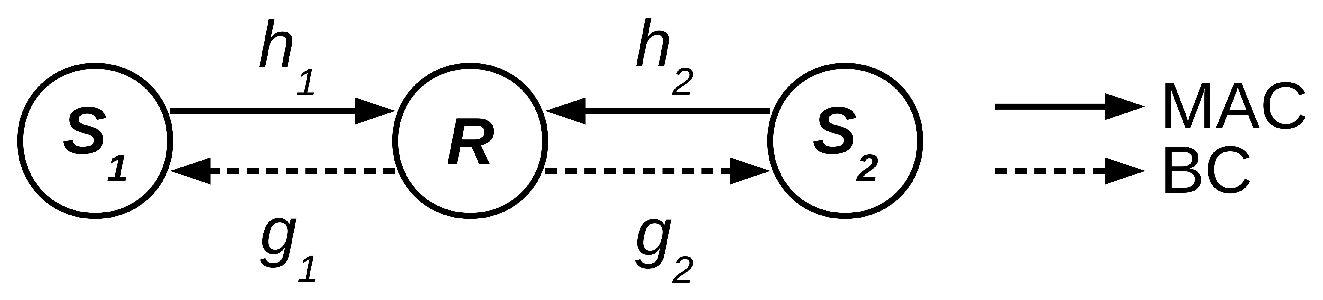
\includegraphics[width=2.0in]{./figs/model.eps}
  \caption{Two-way relay channel with analog network coding.}
  \label{fig:model}
\end{figure}

% Two-way relay channel
Consider a TWRC with analog network coding (ANC) protocol~\cite{choi2013energy}, 
a generalization the AF protocol, as shown in Fig.~\ref{fig:model}. the relay
node $R$ is totally unaware of the HARQ procedure and simply performs ANC. Each round of ANC
transmission is composed of two phases. In the multiple access (MAC) phase, the
two source nodes $S_1$ and $S_2$ transmit to $R$ simultaneously. In the
broadcast (BC) phase, $R$ amplify and broadcast the signal received during the
MAC phase to both $S_1$ and $S_2$.
Denote the uplink channel from $S_i$ to $R$ and downlink channel from $R$ to
$S_i$ as $h_i$ and $g_i$, respectively, where $i=1,2$. We assume that all
the channels follow Rayleigh distribution, i.e.
$h_i\sim\mathcal{CN}(0,\beta_{h_i})$ and $g_i\sim\mathcal{CN}(0,\beta_{g_i})$,
$i=1,2$. Denote the transmitted symbol from $S_i$ as $x_i$ whose average power
$\mathbb{E}[|x_i|^2]=P_i$. Then the signal received by $R$ during the MAC phase
is
\begin{align}
  y_R & = h_1x_1+h_2x_2+n_R,
  \label{eq:y_R}
\end{align}
where $n_r\sim\mathcal{CN}(0,\sigma_R^2)$ is the received noise at $R$. Assuming
that the relay $R$ has an expected power constraint of $P_R$, and that
$S_1$ and $S_2$ perform perfect self-interference cancellation (SIC), then the
received signal at $S_i$ after SIC is
\begin{align}
  y_i &= \alpha g_i y_R + n_i,\;i=1,2,
  \label{eq:y_i}
\end{align}
where $n_i\sim\mathcal{CN}(0,\sigma_i^2)$ is the received noise at $S_i$, and
\begin{align}
  \alpha = \sqrt{\frac{P_R}{|h_1|^2P_1 + |h_2|^2P_2+P_R}}
\end{align}
is the power normalization factor at $R$.

% HARQ protocol
On top of this settings, $S_1$ and $S_2$ performs the HARQ-CC protocol
in an unsynchronized manner. Consequently, the MoDiv design at $S_1$ and $S_2$
can be handled independently. Without loss of generality, we study the HARQ
transmission from $S_1$ to $S_2$. Denote $\mathcal{C}$ as the constellation used
by $S_1$ whose cardinality equals $Q=|\mathcal{C}|$. As a convention, during the
initial transmission of a packet, $S_1$ converts a bit sequence of length
$\log_2Q$ into symbols with Gray mapping $\psi_0:\{0,\ldots,Q - 1\}\rightarrow
\mathcal{C}$. The bit sequence is is labeled by its decimal equivalence $p\in
\{0,\ldots,Q - 1\}$. What distinct HARQ-CC with MoDiv from conventional HARQ-CC
is that, during the $m$-th retransmission, $S_1$ is allowed to use a
mapping function $\psi_m\not=\psi_0$ to remap the same label $p$. We assume
$m \leq M$ where $M$ is the maximum number of retransmissions. According to
Eq.~(\ref{eq:y_R})(\ref{eq:y_i}), the signal received by $S_2$ after SIC during
the $m$-th (re)transmission of $p$ is
\begin{equation}
  y_2^{(m)} = \alpha^{(m)} g_2^{(m)}h_1^{(m)}\psi_m[p] +
  \alpha^{(m)} g_2^{(m)}n_R^{(m)} + n_2^{(m)},
\end{equation}
where $X^{(m)}$ is the $m$-th realization of random variable $X$.

% ML detector
Assume that $S_2$ acquires perfect channel state information
(CSI). After the $m$-th retransmission, it attempts to demodulate the received symbols by
identifying label $p$ with $y_2^{(0)},\ldots,y_2^{(m)}$ via the maximum
likelihood (ML) detection:
\begin{align}
  p^* = \arg\min_p\sum_{j=0}^{m} \frac{|y_2^{(j)} -
  \alpha^{(j)} g_2^{(j)} h_1^{(j)}\psi_j[p]|^2}
  {\sigma_2^2+(\alpha^{(j)})^2\sigma_R^2|g_2^{(j)}|^2}.
\end{align}

\section{Successive Constellation Mapping Design For Modulation Diversity}
\label{sec:modiv}
% Outline

\subsection{A BER upperbound}
\label{ssec:ber}
% The upper bound of BER using PEP

% Recursion of the approximated PEP

\subsection{The Successive Quadratic Assignment Problem}
\label{ssec:qap}
% BER minimization

% Approximated BER minimization

% Successively approximated BER minimization in SQAP form

% Solution via Tabu search


\section{Numerical Results}
\label{sec:numerical}
 % Simulation settings
 
 % Average uncoded BER and BER upperbounds of Non-MoDiv, Seddik, and QAP of for
 % (16) 32 (64) QAM vs d
 
 % Coded BER for 16, (32), 64 QAM for Non-MoDiv, Seddik, and QAP in one graph, M
 % = 3
 
  % Coded BER for 16, (32), 64 QAM for Non-MoDiv, Seddik, and QAP in one graph, M
 % = 4

\section{Conclusion}
\label{sec:conclusion}



% To start a new column (but not a new page) and help balance the last-page
% column length use \vfill\pagebreak.
% -------------------------------------------------------------------------
%\vfill
%\pagebreak

\vfill\pagebreak

% References should be produced using the bibtex program from suitable
% BiBTeX files (here: strings, refs, manuals). The IEEEbib.bst bibliography
% style file from IEEE produces unsorted bibliography list.
% -------------------------------------------------------------------------
\bibliographystyle{IEEEbib}
\bibliography{IEEEabrv,refs}

\end{document}
